%%%% final_report.tex
%% Search Final Project
%% Ryder McMinn

\typeout{Search Final Project}

% Latex Template modified from IJCAI-19 template.

\documentclass{article}
\pdfpagewidth=8.5in
\pdfpageheight=11in
% The file ijcai19.sty is NOT the same than previous years'
\usepackage{ijcai19}

% Use the postscript times font!
\usepackage{times}
\usepackage{soul}
\usepackage{url}
\usepackage[hidelinks]{hyperref}
\usepackage[utf8]{inputenc}
\usepackage[small]{caption}
\usepackage{graphicx}
\usepackage{amsmath}
\usepackage{booktabs}
\urlstyle{same}

% the following package is optional:
%\usepackage{latexsym} 

\title{Search Final Project}

\author{
Ryder McMinn\\
\affiliations
Indiana University - Bloomington\\
\emails
rmcminn@iu.edu
}

\begin{document}

\maketitle

\begin{abstract}
	Code located here:\\ \url{https://github.com/mcminnra/search_final_project}
\end{abstract}

\section*{Introduction}

In this final project, we will attempt two tasks working off the Yelp dataset (\url{https://www.yelp.com/dataset}). In the first task, our goal is be able to predict the categories of a business using textual features. In the second task, I picked applying Youtube's Deep Recommendation approach \cite{youtubedeep} to the Yelp Dataset to be able to recommend businesses to users.

\section*{Task 1 - Multi-Label Classification for Yelp Business Categories}

In this task, our goal is to build a model that is able to predict the categories of a Yelp business. Our approach was to use the text in user reviews plus the business's title to be able to generate predictions of that business's Yelp categories (See Figure \ref{fig:yelp_categories}.)

\begin{figure}[h!]
	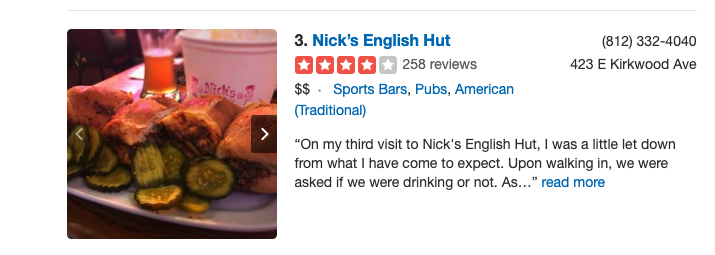
\includegraphics[width=\linewidth]{img/yelp_categories.png}
	\caption{Photo of a local business with it's associated categories.}
	\label{fig:yelp_categories}
\end{figure}

\subsection*{Data Preprocessing}

For task 1, we took a a couple of steps to preprocess the review text before we attempted learning. After some testing, we realized that including the business's title significantly improved performance without affecting preprocessing or training time in any meaningful way. Upon this combination of each review and it's associated business's title, we then removed all punctuation marks and stop words \cite{wiki:stopwords}; removing the punctuation marks allowed us to tokenize the text easier, and removing the stop words deleted words that provided little to no predictive value. This also had the result of speeding up training time, and reducing the training corpus. 

After these steps, we sought to normalize the text. Normalization allows us to reduce the overall corpus by either stemming \cite{wiki:stem} each word to a root spelling or to convert a word to it's associated lemma via lemmatization \cite{wiki:lemma}. This has the effect of reducing training time and increasing accuracy because it more concisely captures a words semantic meaning in all it's various forms, declensions, and conjugations. Looking at Table 1, we can see that stemming is the best approach for our review data. I suspect this has to do with the fact that you lose some semantic meaning with lemmatization. For example, 'great' becomes 'good' and 'awesome' becomes 'good', since 'good' is the lemma of both of these words. However, you lose the information that 'great' and 'awesome' provide. These offer different interpretations of 'good' that have some meaning in the context of a review or business. Losing this information means we lose some predictive value when training. With no word normalization, we then have to train on all the various forms of a word. In this case, we don't lose predictive value, instead, we don't have enough training data to be able to capture all the variations. For example, 'greater', 'greatly', and 'greatness' are all forms of 'great', and if we don't reduce them to just 'great', we need many more examples of each of these to be able to capture the information that 'great' provides. In essence, we may gain some accuracy when we have an immense amount of data, but when we have relatively few examples, it fails to learn each of them, which instead it can learn if we reduce all of them to just 'great'. 

%% Normalization Comparision
\begin{table}[h!]
	\begin{center}
		\caption{Normalization Comparison over 200,000 Reviews (\textbf{Best Results in Bold})}
		\label{tab:table1}
		\begin{tabular}{l||c|c|r} % <-- Alignments: 1st column left, 2nd middle and 3rd right, with vertical lines in between
			\textbf{} & \textbf{Stemming} & \textbf{Lemmatization} & \textbf{None}\\
			\hline
			Preprocessing (min.) & \textbf{21.06} & 25.16 & 27.58\\
			Training (min.) & \textbf{13.55} & 14.58 & 14.86\\
			Train Loss & .0048 & .0048 & \textbf{.0047}\\
			Validation Loss & \textbf{.0070} & .0071 & .0071\\
			Test Loss & \textbf{.0069} & .0070 & .0071\\
		\end{tabular}
	\end{center}
\end{table}

After normalization, we converted our reviews to a sequence of word ids and padded them with zeros, so they are all the same length. This will allow us to do convolutions over our text data (e.g. [14, 23, 2, 67, 0, 0, 0, 0])

\subsection*{Approach and Architecture}

Our approach to predicting these categories was to use trained word embeddings and then apply a convolution layer over them (See Architecture below)

\mbox{}\\
\begin{verbatim}
Embedding Layer (length=50)
\end{verbatim}
$\downarrow$
\begin{verbatim}
1-D Convolution Layer
(filters=128,
 filter_size=5,
 activation='relu')
\end{verbatim}
$\downarrow$
\begin{verbatim}
Global Max Pooling Layer
\end{verbatim}
$\downarrow$
\begin{verbatim}
Dense Layer (neurons=1000)
\end{verbatim}
$\downarrow$
\begin{verbatim}
Softmax Output(1300 categories)
\end{verbatim}
\mbox{}\\

We trained our output layer using Binary Crossentropy loss in order to be able to learn multiple categories (Multi-Label) on output. From personal experience if each text example is short (like a review), and contains natural spoken speech patterns, the best approach is to simply use the above architecture of WordEmbeddings+CNN. I tried to add an LSTM layer, but since most reviews were short and contained natural speech, the LSTM had trouble finding key dependencies to remember that would improve performance. The result was significantly increasing training time, while not improving the loss. I, also, tried using a simple Multi-Layer Perception with TFIDF features, but the feature size grew exponentially large, and made meaningful training impossible. Memory became a huge bottleneck and prohibited using large data sizes for training

\subsection*{Results}

Here you'll see my best model results. I ran out of time to do comparisons to previous iterations and techniques unfortunately. This is taken as an average of each category (class) individually since we used a multi-label approach.  

%% Best Results
\begin{table}[h!]
	\begin{center}
		\caption{Best Results over Test Set of 199934 reviews}
		\label{tab:table1}
		\begin{tabular}{l|r} % <-- Alignments: 1st column left, 2nd middle and 3rd right, with vertical lines in between
			\textbf{Metrics} & \textbf{Test Set}\\
			\hline
			Loss & 0.0048\\
			Accuracy & 0.9986\\
			Average Macro Precision &  0.6095\\
			Average Macro Recall &  0.3601\\
			Average MCC & 0.4507\\
		\end{tabular}
	\end{center}
\end{table}

In this problem, we want to pay attention to precision more than recall. We care more about trying to predict relevant categories than we care about predicting all the relevant categories. In our case, it's better for a business to be unlabeled than to be mislabeled. If we look at MCC, we can see our model performs well, but there is quite a bit of room for improvement. Below there is a random sample of businesses and our predicted categories for them. 

\begin{verbatim}
Predicted Categories: ['Restaurants']
Real Categories: 
['Restaurants', 'Seafood', 'Steakhouses']

Name: Ah-So Sushi & Steak
Predicted Categories: 
['Sushi Bars', 'Steakhouses',
 'Japanese', 'Restaurants']
Real Categories: ['Japanese', 'Restaurants']

Name: Chang's Hong Kong Cuisine
Predicted Categories: 
['Cantonese', 'Diners', 'Seafood', 
'Dim Sum', 'Chinese', 'Restaurants']
Real Categories: 
['Cantonese', 'Chinese', 'Dim Sum', 
'Diners', 'Restaurants', 'Seafood']

Name: Sushi Wa
Predicted Categories: 
['Japanese', 'Sushi Bars', 'Restaurants']
Real Categories: 
['Japanese', 'Restaurants', 'Sushi Bars']

Name: Rancho Pinot
Predicted Categories: 
['Mexican', 'Restaurants']
Real Categories: 
['American (New)', 'Bars', 
'Italian', 'Nightlife', 'Restaurants', 
'Wine Bars']
\end{verbatim}

\subsection*{Future Work}

There is a lot that can be done to our approach to improve performance. Firstly, we use very little in the way of features. We only use review text and the business name. We can include location information, rating stars, various review attributes, etc. I believe if we had more time and less scrubbed data, we could build a much better performing model. Secondly, we can leverage more complex models and increased number of training data. I limited myself to a small subset of the data in interest of time, but in a real-world environment, we could train longer and possibly see more performance. As an aside, most the concepts and techniques I personally learned was from the Deep Learning \cite{Goodfellow-et-al-2016} textbook. 

\pagebreak

\section*{Task 2 - Deep Recommendation}

In this task, our goal was to apply Youtube's Deep Recommendation approach \cite{youtubedeep} to yelp businesses. We have each User, businesses they've rated, and the stars they gave it in order to hopefully learn a relation between users and businesses, so we can leverage them to make recommendations. 

\subsection*{Data Preprocessing}

Data Preprocessing for this task was reletively simple. As we needed was to merge user ids and business ids together with the stars they gave that business. This means we may have multiple samples of a single user that each contain a different business it has reviewed. Finally since each id is an alphanumeric string, I converted them to a single integer index for training.

\subsection*{Approach and Architecture}

Our approach to generating these recommendations is to learn embeddings for both the user and the business, then concatenate them together so we can feed them into dense layers. As an output, we produce a single integer presenting the stars we believe the user would rate the business. We can then use this stars output to rank each business. (See Architecture Below)

\mbox{}\\
\begin{verbatim}
User Embedding Layer (length=50)
\end{verbatim}
$+$
\begin{verbatim}
Business Embedding Layer (length=50)
\end{verbatim}
$\downarrow$
\begin{verbatim}
Dense Layer (neurons=512)
\end{verbatim}
$\downarrow$
\begin{verbatim}
Dropout Layer (0.2 dropout rate)
\end{verbatim}
$\downarrow$
\begin{verbatim}
Dense Layer (neurons=256)
\end{verbatim}
$\downarrow$
\begin{verbatim}
Dropout Layer (0.2 dropout rate)
\end{verbatim}
$\downarrow$
\begin{verbatim}
Dense Layer (neurons=128)
\end{verbatim}
$\downarrow$
\begin{verbatim}
Output Layer (single value)
\end{verbatim}
\mbox{}\\

\subsection*{Results}

Below is two randomly sampled users, see the issue?

\begin{verbatim}
User 1:
\end{verbatim}

\begin{verbatim}
User 2:
\end{verbatim}
\subsection*{Future Work}

\medskip

\bibliographystyle{unsrt}
\bibliography{final_report}

\end{document}